\documentclass[fleqn]{article}

\usepackage{amsmath, latexsym, amssymb, mathtools}
\usepackage{mathptmx}
\usepackage{fontspec}
    \setsansfont{AppleSDGothicNeo-Regular}[BoldFont = AppleSDGothicNeo-Bold]
    \setmainfont{TimesNewRomanPSMT}[ItalicFont = TimesNewRomanPS-ItalicMT, BoldFont = TimesNewRomanPS-BoldMT, BoldItalicFont = Times-RomanSC]
\usepackage{tabularx}
    \newcolumntype{C}{>{\centering\arraybackslash}X}
\usepackage{tikz}
    \tikzset{every node/.append style = {font = \small}, > = latex}
\usepackage[ruled]{algorithm2e}
\usepackage{etoolbox}
    \AtBeginEnvironment{algorithm}{\let\textnormal\ttfamily}
\usepackage{sectsty}
    \sectionfont{\large\bfseries}
    \subsectionfont{\normalsize\bfseries}
\usepackage{geometry}
    \geometry{
    a4paper,
    total={150mm, 240mm},
    left=30mm,
    top=30mm,
    }

\renewcommand{\figurename}{Figure}
\allowdisplaybreaks

\begin{document}
\begin{center}
    \large\bfseries M1522.000800 System Programming\\
    Fall 2019\\
    \Large\normalfont\bfseries\itshape System Programming Memory Lab Report
\end{center}
\begin{flushright}
    Dept. of statistics, 2015-10283, Sanghyun, Park.
\end{flushright}

\section{Introduction}
The goal of this lab is to implement malloc package that dynamically allocates and frees heap memory. With this lab, we can improve our understanding of dynamic memory allocation and heap management. Also, it is a good chance to handle trade-off relation between memory utility and throughput.

\section{Important Concepts}

In this section, I shall introduce some of main concepts regarding this memory lab.

\subsection{Dynamic memory allocator}

As we learned in class, physical memory is managed by MMU and OS. They allocate when the process needs more memory and retrives it when it is of no more use. However, the unit of management is page which is at least 4KB. Thus it cannot handle memory regions whose size is less than 4KB. In this situation, \textit{dynamic memory allocator} plays its role. By allocating and freeing memory with various size dynamically, it can further efficiently manange memory resources. The main two functionality of dynamic memory allocator is malloc (memory alloction) and free. In this lab, these two functionality is to be implemented.

\subsection{Throughput and memory utilization}

As mentioned, dynamic memory allocator manages memory resources. And there are some barometers to measure how efficiently they work. Two of them is \textit{throughput} and \textit{utilization}. Throughput is measurement if fastness, which is defined by the number of completed malloc and free requests per unit time. Since memory operations are relatively expensive, but essential to almost every program, it should be fast enough. On the other hand, utilization is measurement of memory efficiency. For various reasons, it is very difficult and almost impossible to use memory 100\% meaningfully. Some parts of memory is fragmented which drops memory efficiency. Thus good dynamic memroy allocator should minimize such cases. There are various measrues of utilization, and in this lab we use \textit{peak utilization ratio} whose definition can be found at textbook or instruction PDF.

The problem is, these two main measurements are often trade-off with each other. Thus if one maximizes throughput, then utilization becomes poor and vice versa. Thus we need a proper blance between these two.

\subsection{Segmented list}

\textit{Segmented list} is one of data structure used to manage heap memory. The idea is to make search for free block fast by grouping block of simliar sizes. Usually, size is divided into some ranges, which is called \textit{bin}, whose size and number varies. Every free blocks lies in exactly one bin and free blocks in a bin is somehow linked to each other. With this data structure, we can make free block searching process much faster and also memory utilization improves. The detailed implementation of segmented list in my \texttt{mm.c} will be explained in detail in following sections.

\section{Structure}

In this section, I shall explain the global organization of heap and data structures used for implementation.

\subsection{Heap structure}

\begin{figure}[ht!]
    \centering
    \includegraphics[width = 0.7\textwidth]{global_struct}
    \caption{Global structure of heap}
\end{figure}

Heap starts with 8 word size (32bytes) \textit{micro memory} region. This region is specially reserved for storing some statistics on malloc requests. I can noticeably improve memory utilization with those statistics, so that overhead of 32bytes is justified. I shall explain on memory utilization optimization tricks later in detail. Then 13 \textit{prologue blocks} for segmented list follows. To minimize internal framentation, prologue blocks do not have header, so it is 3 word (12bytes) size each. Thus 13 prologue blocks sums up to 156bytes. With those prologue blocks, implementation of operations on segmented lists, like search, insertion, and deletion becomes much elegant. I shall present the code in following sections. Then the heap region for allocated or freed blocks follows. At the end of heap, I placed 13 \textit{epilogue blocks} for segmented lists, each of 3 word (12bytes) ommiting footers this time, to minimize internal fragmentation. As shown at the figure 1, there are three static pointers \texttt{micro\_memp}, \texttt{segl\_prolp} and \texttt{segl\_epilp} pointing to the starting address of each region.

\subsection{Block structure}

\begin{figure}[ht!]
    \centering
    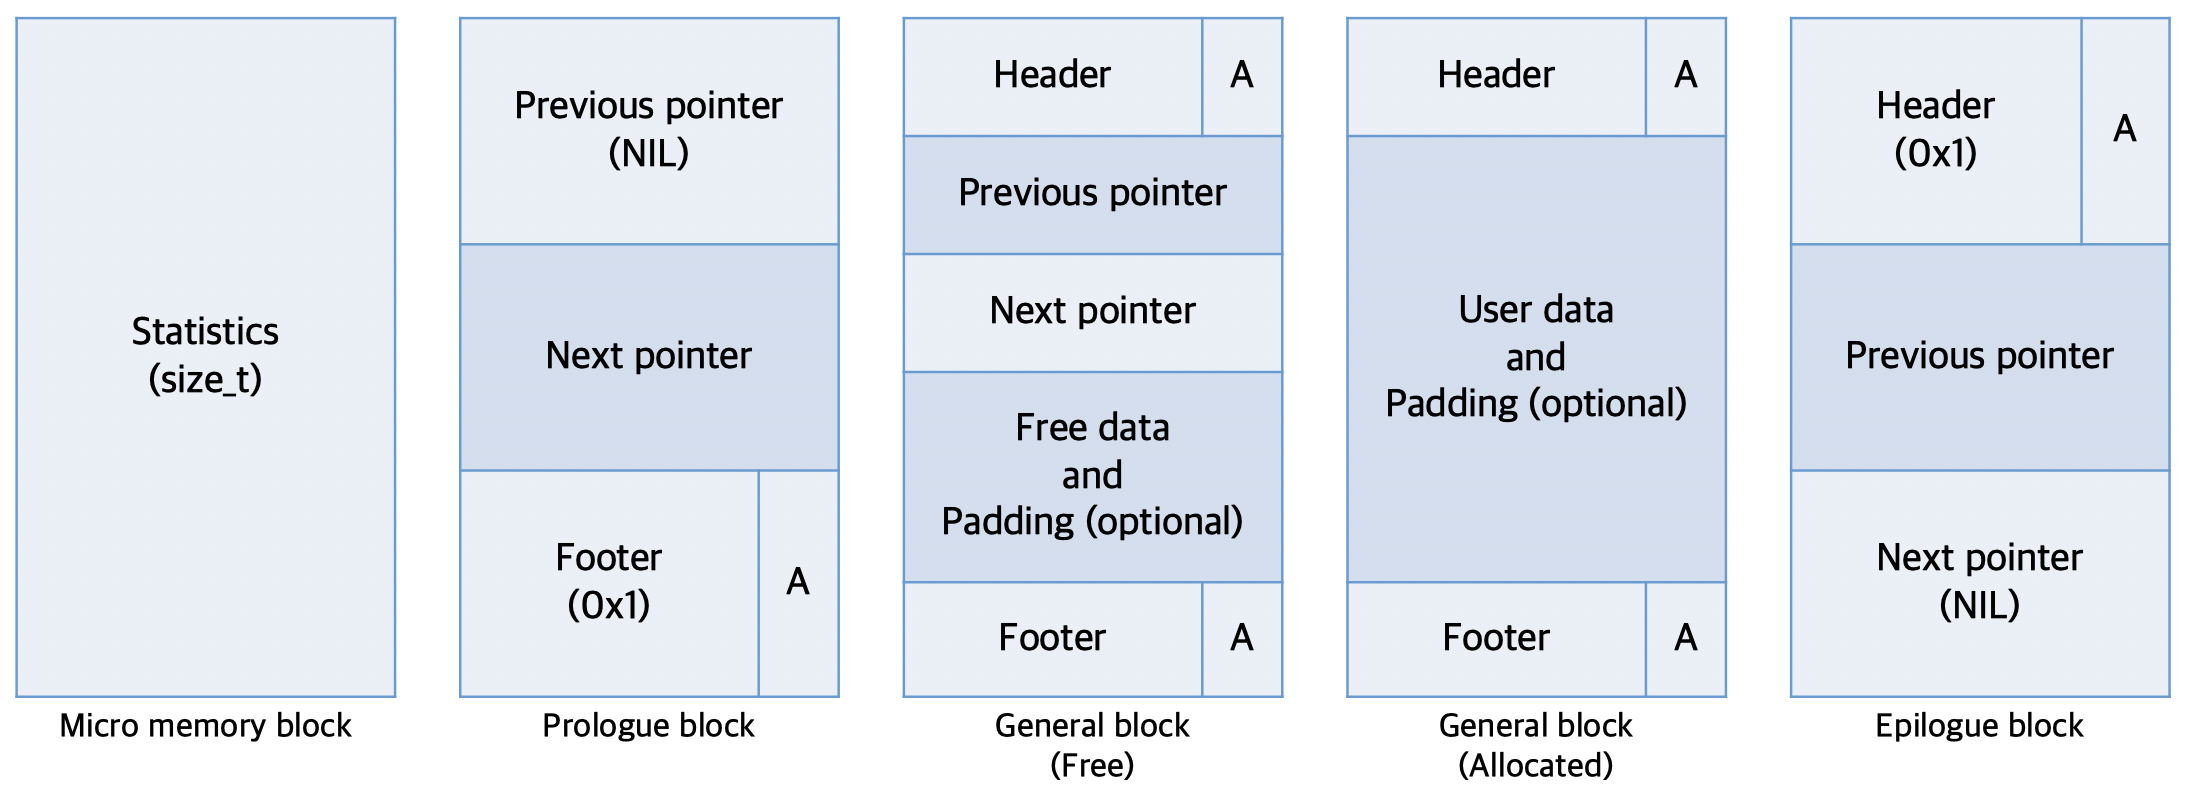
\includegraphics[width = 0.8\textwidth]{block_struct}
    \caption{Structure of blocks}
\end{figure}

There are total four kinds of blocks. First one is \textit{micro memory blocks}. Literally, they comprises micro memory region. Since micro memory region is only used for storing statistics, it is simple one word size (size of \texttt{size\_t}) block with no further structures. Although they are not linked by pointers, I can refer them using \texttt{micro\_mem} pointer since micro memory region is static array of fixed size.

Blocks that actually store user data has structure of \textit{general blocks} in the figure 2. Following the standard version of segmented list implementation, general blocks consists of four parts: header, previous pointer, next pointer, and footer which are all one word size each. In case of free blocks, they have all four parts where some free space lies between next pointer and footer. In case of allocated blocks, user data will override previous and next pointer part since those are only needed for free blocks. This shall lightens the burden of strutural overhead of segmented list. As usual, header and footer contains size of its block in bytes. Since blocks are following double word (8bytes) alignment rule, the 3 LSB is not used. So I placed the allocated bit at LSB of header and footer: 1 for allocaed and 0 for free.

As mentioned, \textit{prologue blocks} and \textit{epilogue blocks} are almost identical with (free) general blocks with one difference: absence of header and footer, respectively. Although ommited header and footer helps decreasing internal fragmentation, I should care more for pointer operations in segmented list because refering non-existing header and footer mainly causes perflexing segmentation faults. To present the begining of segmented list, previous pointer and footer of prologue block will be always set as \texttt{NIL} and \texttt{0x1}. (Footer and header \texttt{0x1} implies 0 bytes size which is allocated. Marking prologue and epilogue blocks as allocated keeps coalescing logic simple but elegant.) In similar fashion, epilogue block's header and next pointer will be always set as \texttt{0x1} and \texttt{NIL}, respectively.

Note that with above global structure and block design, there is no need for additional padding blocks. Indeed, if we assume our heap starts at \texttt{0x0}, the first general block will lie at \texttt{0xc0} which is automatically aligned. In fact, the global structure and block design are carefuly organized to eliminate chumbersome padding blocks beforehand.

\subsection{Segmented list}

\begin{figure}[ht!]
    \centering
    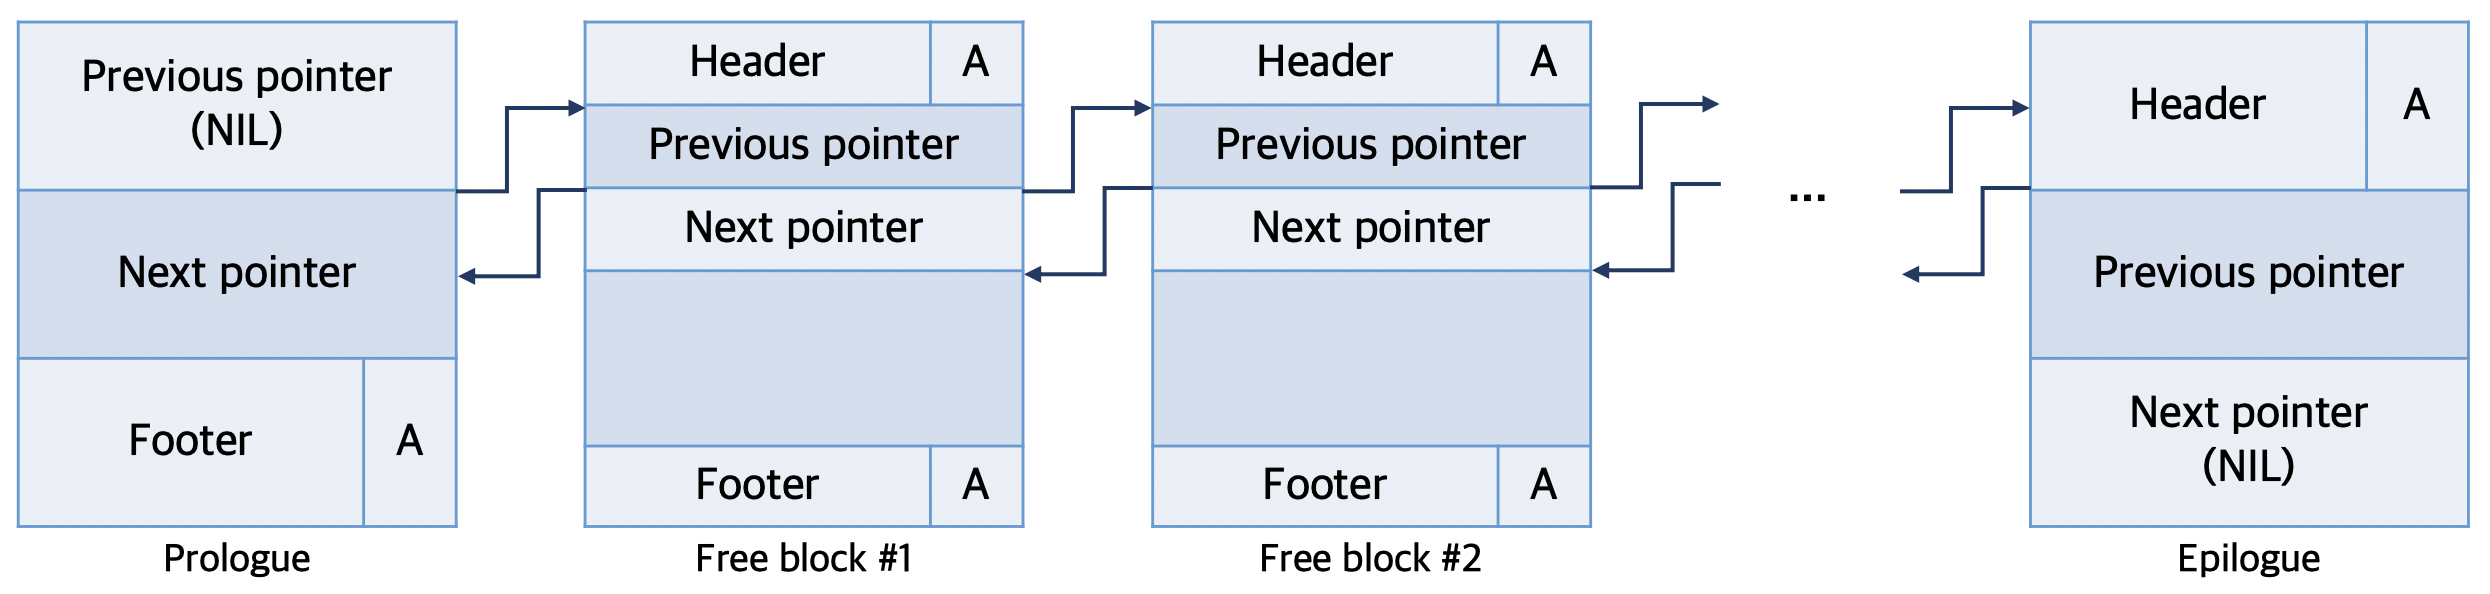
\includegraphics[width = 0.8\textwidth]{segl_struct}
    \caption{Structure of segmented list}
\end{figure}

I organized 13 equivalent classes each ranges as following table. Every free block is contained in exactly one class and equivalent free blocks are linked by previous and next pointers. Standard doubly linked list structure is employed for implementation, so that we can traverse back and forth freely in an equivalence class following those links. As one might noticed, each equivalence class has its one prologue and epilogue blocks (hence total 13) and the next pointer of prologue block points to the first free block while the last free block is pointed by the previous pointer of epilogue block.

\vspace{1em}
\noindent
\begin{tabularx}{\textwidth}{c|CCCCCCC}
    \hline
    Index of bin & 0 & 1 & 2 & 3 & 4 & 5 & 6\\
    \hline
    Size range & $[0,\,2^5)$ & $[2^6,\,2^7)$ & $[2^7,\,2^8)$ & $[2^8,\,2^9)$ & $[2^9,\,2^{10})$ & $[2^{11},\,2^{12})$ & $[2^{12},\,2^{13})$\\
    \hline
    \hline
    Index of bin & 7 & 8 & 9 & 10 & 11 & 12 &\\
    \hline
    Size range & $[2^{13},\,2^{14})$ & $[2^{14},\,2^{15})$ & $[2^{15},\,2^{16})$ & $[2^{16},\,2^{17})$ & $[2^{17},\,2^{18})$ & $[2^{18},\,\infty)$ & \\
    \hline
\end{tabularx}

\section{Algorithm}

In this section, I shall explain algorithms and optimization tricks used in my \texttt{mm.c}.

\subsection{Find-fit}

When the user calls \texttt{mm\_malloc}, it starts searching at equivalence class of appropriate size, which is $\log_2$ of requested size minus 4. Of course, to meet alignment, allocating size is rounded up to the nearest multiple of 8. For find-fit policy, I adopted the \textit{best-fit} approach. Inside an equivalence class, it searches the best-fit block for request. If there is a free block of exact fit, then it immediately terminate searching process. Otherwise, it searches the whole list and after that, returns the smallest free block which can afford the user request. If there is no affordable free block at all, then it recursively calls search procedure for the next level equivalence class. In case of search ultimately fails after all recursive calls, which is very unfortunate, it extend the heap using \texttt{mem\_sbrk}. Although this appraoch has linear time complexity, thanks to coalesing and segmented list, it does not eat up throughput severely. Indeed, the throughput part of performance index is 30, which is as fast as always-heap extending approach. In my \texttt{mm.c}, it is implemented as a function \texttt{segl\_find}.

\small
\begin{verbatim}
size_t *segl_find(size_t size, unsigned int idx) {
    // Search failed
    if (idx >= BIN_CNT) return NULL;
    
    size_t *find = NULL;
    size_t *bp;
    size_t min = UINT_MAX;

    // Loop all blocks in bin to find best fit
    for (bp = NEXT_FREE_BLKP(FIRST_PROL_BLKP(idx));
        GET_SIZE(HDRP(bp)) > 0; bp = NEXT_FREE_BLKP(bp)) {
        // If there is an exact fit, immediately return
        if ((GET_SIZE(HDRP(bp))) == size) return segl_pop(bp);

        // If there is block large enough, record it
        if ((GET_SIZE(HDRP(bp)) >= size) && (GET_SIZE(HDRP(bp)) < min)) {
            find = bp;
            min = GET_SIZE(HDRP(bp));
        }
    }

    // If there is at least one good fit, then return
    if (find != NULL) return segl_pop(find);

    // Otherwise, continue search at next level
    return segl_find(size, idx + 1);
}
\end{verbatim}
\normalsize

\subsection{Placing}

After getting afordable free block, it deletes the free block from segmented list if it is found in segmented list. Then it calls another procedure takes care of placing judgement. Based on the size of request and size of free block, it \textit{alwalys splits}. Note that the smallest possible general block size is 4 word size (16bytes). Thus if the difference between the free block size and requested size is greater than 16 bytes, then it splits. Splitted block immediately goes back to the segmented list. In my \texttt{mm.c}, it is implemented as a function \texttt{place}.

\small
\begin{verbatim}
size_t *place(size_t *bp, size_t size) {
    size_t csize = GET_SIZE(HDRP(bp));
    size_t *split;

    if ((csize - size) < 2 * DSIZE) {
        // If current block size is not big enough, just place and return
        SET_HDR(HDRP(bp), csize, ALOC);
        SET_FTR(FTRP(bp), csize, ALOC);
    } else {
        // Otherwise, split
        SET_HDR(HDRP(bp), size, ALOC);
        SET_FTR(FTRP(bp), size, ALOC);
        split = NEXT_BLKP(bp);
        SET_HDR(HDRP(split), csize - size, FREE);
        SET_FTR(FTRP(split), csize - size, FREE);
        segl_push(split);
    }

    return bp;
}
\end{verbatim}
\normalsize

\subsection{Coalescing}

Coalescing is at the heart of optimization. After plenty of trial and errors, I adopted a \textit{selective coalescing}. Coalescing has pros and cons which is somehow interacts in intricate way. At first glance, coalescing makes free blocks larger, thus eliminating false fragmentation. But there is a pithole. Too much coalescing makes large and small blocks mix up together, which may cause serious external fragmentation. (Mixing up various size of blocks are not good. For example, small blocks which has long life between large blocks which has very short life keeps large chunk of free blocks from coalescing. This phenomenon stands out in trace file \texttt{binary-bal.rep}.) So there is somehow complicated determination logic regarding coalescing.

\begin{itemize}
    \item If free block is achived by user call \texttt{mm\_free}, then immediately coalesce.
    \item If free block is achived by extending heap, then based on the size of the last allocated block, it either coalesces or not. If the size of the last allocated block is larger than the half of newly extended heap size, then coalesce. Otherwise, do not. The idea of this trick is to keep small blocks nearby each other.
\end{itemize}

In my \texttt{mm.c}, this trick is implemented as a part of \texttt{extend\_heap}.

\small
\begin{verbatim}
// Selectively coalesce extended heap
if (!empty_flag) {
    lbp = LAST_BLKP;
    
    // First, handle some marginal cases
    if (GET_ALOC(HDRP(lbp))) {
        size = MAX(size, chunksize);
        coal = 0;
    } else if (GET_VAL(PREV_BLKP_FTRP(lbp)) == 0) {
        size = size - GET_SIZE(HDRP(lbp));
        coal = 1;
    } else if (GET_SIZE(HDRP(PREV_BLKP(lbp))) < (size / 2)) {
        // If the last allocated block is small relatively, do not coalesce
        size = MAX(size, chunksize);
        coal = 0;
    } else {
        // If the last allocated block is large relativley, then coalesce
        size = size - GET_SIZE(HDRP(lbp));
        coal = 1;
    }
} else {
    // If heap is empty, then cannot coalesce
    size = MAX(size, chunksize);
    coal = 0;
}
\end{verbatim}
\normalsize

\subsection{Free}

Free is rather simple. After checking the validity of free request to prevent double free error, it immediately frees the requested block. Then the freed block goes into the segmented list. Since they will be inserted as the first member of list, it is a constant time operation which can be done very fast.

\small
\begin{verbatim}
void mm_free(void *ptr) {
    // If one tries to double free abort
    if (!GET_ALOC(HDRP(ptr))) {
        printf("Double free\n");
        exit(EXIT_FAILURE);
    }

    size_t size = GET_SIZE(HDRP(ptr));

    SET_HDR(HDRP(ptr), size, FREE);
    SET_FTR(FTRP(ptr), size, FREE);
    segl_push(coalesce(ptr));

    /* DON'T MODIFY THIS STAGE AND LEAVE IT AS IT WAS */
    if (gl_ranges) remove_range(gl_ranges, ptr);
}
\end{verbatim}
\normalsize

\subsection{heap extension}

Another optimization trick lies in heap extension. Again, the idea is keeping small blocks nearby each other. This can be done by adjusting minimum size of heap extension. Also, extending heap properly large is good for throughput since it replaces frequent heap extension for small size which is relatively slow. The hard part is determining `proper large size'. In each application, the proper size must be different, so it cannot be hard coded. And based on our expreience and coding convention, we know that there are some rare but extreme allocation requests. If we adjust the minimum size to be the maximum request so far, then such an extreme rare event will cause catastrophic senario, ending up poor utilization or even running out all available memory. Further, there is so called the 'trend' of request. Some applications makes lots of malloc requests in initialization step and after initailization, it just requests small tiny bytes.

In this situation, my other major, statitsics plays it role. At every malloc request, it records the size of request in micro memory. And at every 8th request, it stops the allocating process for a while and estimates `proper large size' and update the minimum heap extensino size. After some thought and couple of experiments, estimator is choosen to be the second maximum. Statistically, order statistics are much robust (does not affected by outliers) and choosing the second maximum, not maximum makes it more robust. In addition to this, since it is re-estimated for every 8 cycle, it automatically follows the trend of request. Computationally, algorithm finding second minimum can be implemented using very simple one-pass algorithm, keeping high throughput. Combined with selective coalescing trick, the result is very promising, improving average utilization from 86\% to 94\%. (For 2 trace files, utilization reached 100\% and for \texttt{binary-bal.rep}, it showed almost improvement of 40\%p.) In my \texttt{mm.c}, this trick is implemented as a function \texttt{micro\_sched}.

\small
\begin{verbatim}
void micro_sched(void) {
    int i;
    size_t max = 0, second_max = 0;
    size_t temp;

    // Find second maximum
    for (i = 0; i < MICRO_MEM_CNT; i++) {
        temp = READ_MICRO_MEM(i);
        if (max < temp) {
            max = temp;
        } else if (second_max < temp) {
            second_max = temp;
        }
    }

    // Update chunksize
    chunksize = ALIGN(second_max);
}
\end{verbatim}
\normalsize

\section{Conclusion}

As a result, preformance index of my \texttt{mm.c} reached 96 points (66 for utilization and 30 for throughput), which is (personally) quite satisfying. For me, this lab was somehow fun. Optimizing throughput and memory utilization requires couple of days to think deeply. It took a long time, but was fruitful. During this lab, I read some articles regarding dynamic memory allocator like dlmalloc. Although I do not used any idea directly, it helps me to widen my thoughts and concepts like desginated victim in dlmalloc provided precious insights.

One can make even further improvement. One can organize each equivalence classes using self-balancing tree (eg. AVL tree or RB tree) instead of doubly linked list. It may make the source code somehow more complex, but with this structure, one can theoretically ensure the log time complexity for best-fit search for free blocks. One can improve external fragmentation further. As one might noticed from the name of function \texttt{micro\_sched}, we can `macro schedule' the malloc requests. Unfortunately theses ideas are not implemented in my \texttt{mm.c} because of limited time.

\end{document}